%%%%%%%%%%%%%%%%%%%%%%%%%%%%%%%%%%%%%%%%%%%%%%%%%%%%%%%%%%%%%%%%%%%%%%%%%%%%%%%%
%% Document Setup
%%%%%%%%%%%%%%%%%%%%%%%%%%%%%%%%%%%%%%%%%%%%%%%%%%%%%%%%%%%%%%%%%%%%%%%%%%%%%%%%
%%% This document is processed in an isolated clean folder at the same level.
\makeatletter
\def\input@path{{../tex/}}
\makeatother
%%% Include the preamble at choice during processing.
\documentclass[a4paper,10pt]{report}

%% This document is processed in an isolated clean folder at the same level
\makeatletter
\def\input@path{{../tex/}}
\makeatother

%% Page settings
%%% \usepackage[margin=0.5in,nomarginpar]{geometry}

%%% Bibliography system setup using biblatex
\usepackage[
    backend=biber,
    style=alphabetic,
]{biblatex}
\addbibresource{../tex/Biblio.bib}

%% Packages
\usepackage[utf8]{inputenc}
\usepackage{hyperref}
\usepackage{fvextra}
\usepackage{csquotes}
\usepackage{xcolor}
\usepackage{minted}
\usepackage{amsfonts}
\usepackage{amsmath}
\usepackage{graphicx}
\usepackage{enumitem}

%% Formatting

\renewcommand{\mkbegdispquote}[2]{\itshape}

%% Required Literate Haskell (lhs) macros (code, spec)
%%% include common lhs formatting
\input{lhsfmt.tex}
%%% for code
\newminted[code]{haskell}{}
\newminted[spec]{haskell}{}

%% Other macros
\long\def\ignore#1{} % for ignoring code
\newcommand{\eg}{\textit{e}.\textit{g}.}
\newcommand{\ie}{\textit{i}.\textit{e}.}
\newcommand{\etal}{\textit{et al}.}

%% Used Unicodes in code
\DeclareUnicodeCharacter{03BD}{$\nu$}
\DeclareUnicodeCharacter{2205}{$\emptyset$}
\DeclareUnicodeCharacter{2295}{$\oplus$}
\DeclareUnicodeCharacter{27E6}{$[\![$}
\DeclareUnicodeCharacter{27E7}{$]\!]$}
\DeclareUnicodeCharacter{1D4DC}{$\mathcal{M}$}

%%% Bibliography system setup using biblatex.
\usepackage[
    backend=biber,
    style=alphabetic,
]{biblatex}
\addbibresource{../tex/Biblio.bib}
%%% Macros used.
\long\def\ignore#1{} % for ignoring some code
\newcommand{\eg}{\textit{e}.\textit{g}.}
\newcommand{\ie}{\textit{i}.\textit{e}.}
\newcommand{\etal}{\textit{et al}.}

%%%%%%%%%%%%%%%%%%%%%%%%%%%%%%%%%%%%%%%%%%%%%%%%%%%%%%%%%%%%%%%%%%%%%%%%%%%%%%%%
%% Document Meta Data
%%%%%%%%%%%%%%%%%%%%%%%%%%%%%%%%%%%%%%%%%%%%%%%%%%%%%%%%%%%%%%%%%%%%%%%%%%%%%%%%

\title{Denotational Semantics of General Payment Primitives, and Its Payment System}

\author{\\
    Miao, ZhiCheng\\
    Co-Founder, Superfluid Finance\\
    miao@superfluid.finance
}

%%%%%%%%%%%%%%%%%%%%%%%%%%%%%%%%%%%%%%%%%%%%%%%%%%%%%%%%%%%%%%%%%%%%%%%%%%%%%%%%
%% Document Body
%%%%%%%%%%%%%%%%%%%%%%%%%%%%%%%%%%%%%%%%%%%%%%%%%%%%%%%%%%%%%%%%%%%%%%%%%%%%%%%%
\begin{document}
\maketitle

\begin{abstract}
    \begin{center}
        (Some distant lyrics as the placeholder for the actual abstract)

        Money, money, money

        Must be funny

        In the rich man's world

        Money, money, money

        Always sunny

        In the rich man's world

        \

        Ah, all the things I could do

        If I had a little money

        It's a rich man's world

        It's a rich man's world
    \end{center}
\end{abstract}

%%%%%%%%%%%%%%%%%%%%%%%%%%%%%%%%%%%%%%%%%%%%%%%%%%%%%%%%%%%%%%%%%%%%%%%%%%%%%%%%%%%%%%%%%%%%%%%%%%%%%%%%%%%%%%%%%%%%%%%%
\chapter{Introduction}
%%%%%%%%%%%%%%%%%%%%%%%%%%%%%%%%%%%%%%%%%%%%%%%%%%%%%%%%%%%%%%%%%%%%%%%%%%%%%%%%%%%%%%%%%%%%%%%%%%%%%%%%%%%%%%%%%%%%%%%%

It should be fair to say, every aspect of money are controversial: the nature of money, the value of money, money and
banking, and monetary reconstruction. Two major schools of thoughts about theory of money are the \textit{Austrian
    school} (\cite{von2013theory}) and the \textit{Chicago school} (\cite{friedman1989quantity}). That is before the
appearance of Internet-era version of monetary reconstruction, broadly defined as cryptocurrency, which challenges
theories of money further and demands their updates (\cite{ammous2018can} \cite{hardle2020understanding}).

This yellow paper does not intend to address these controversies, but to focus on the function of money. According to
Von Mises:

\begin{displayquote}
The function of money is to facilitate the business of the market by acting as a common medium of
exchange. \footfullcite[][Chapter One, Chapter I, § 1, p1]{von2013theory}
\end{displayquote}

How do different forms of money perform this function, especially in the information age, when electronic forms of money
are increasingly used?

This paper adds a new controversy to money, that is to present a survey challenging the preconceived notion of how money
can perform its function of medium of exchange.

In Chapter 2, we shall first explore the foundation for the survey. Here we present a formal definition of payment
system and its components. We then select a few relevant approaches used in computer science useful for modeling and
defining formal specification for the payment system.

One of the approaches is \textit{denotational semantics}, which is used in Chapter 3 of the paper to define the general
payment primitives. Along with the denotational semantics, a restatement\footnote{It is a borrowed term from common law:
"restatement of the law". In our case, the denotative mathematical "laws".} of it in \textit{Haskell programming
    language} (\cite{hudak1992report} \cite{jones2003haskell} \cite{marlow2010haskell}) is also included.

In Chapter 4, a reference implementation of the general payment primitives and its payment system called
\textit{Superfluid Money} is introduced.

In Chapter 5, some possible further investigations are included for future study purpose.

%%%%%%%%%%%%%%%%%%%%%%%%%%%%%%%%%%%%%%%%%%%%%%%%%%%%%%%%%%%%%%%%%%%%%%%%%%%%%%%%%%%%%%%%%%%%%%%%%%%%%%%%%%%%%%%%%%%%%%%%
\chapter{Foundation}
%%%%%%%%%%%%%%%%%%%%%%%%%%%%%%%%%%%%%%%%%%%%%%%%%%%%%%%%%%%%%%%%%%%%%%%%%%%%%%%%%%%%%%%%%%%%%%%%%%%%%%%%%%%%%%%%%%%%%%%%

%%%%%%%%%%%%%%%%%%%%%%%%
\section{Payment System}
%%%%%%%%%%%%%%%%%%%%%%%%

Here we present a definition of payment system and its components.

\paragraph{Payment system}

It can be solely defined by these components:

\begin{itemize}
\item \textit{money distribution} models how monetary value is distributed amongst bearers\footnote{(Banking \& Finance)
a person who presents a note or bill for payment. - Collins English Dictionary},
\item \textit{payment primitives} updates money distribution,
\item \textit{payment execution environment} performs payment primitives,
\item and \textit{forms of money medium} are the "user interfaces" of money for the bearers.
\end{itemize}

\paragraph{Modernization}

For its modern upgrade, the system should also have these properties:

\begin{itemize}
\item Money can be distributed continuously over time, as opposed to be discrete.
\item Payment primitives can involve more than two parties, as opposed to be only for a sender and a receiver.
\item Financial system should be compositional.
\end{itemize}


\subsection{Money Distribution}
%%%%%%%%%%%%%%%%%%%%%%%%%%%%%%%

A representation of money and its distribution proposed in \cite{buldas2021unifying} involves the following components:

\begin{itemize}
\item U is the set of monetary units.
\item $\nu : U \rightarrow \mathbb{N}$ is the value function defining the value $\nu(u)$ of every value unit u. The set
    $\mathbb{N}$ is the set of all natural numbers, but instead, we can use any set of numerals that is totally ordered
    (\eg\ integers, real numbers).
\item $\beta : U \rightarrow \mathfrak{B}$ is the bearer function defining the bearer $\beta(u)$ of a unit. The set
    $\mathfrak{B}$ is the set of possible bearers. The bearer is usually a legal construction defining any type of legal
    entity, such as a person, a family, a company, a state institution, etc.
\end{itemize}

This discrete nature of this money distribution model is schematically depicted in \ref{fig:discrete-md}:

\begin{figure}[h]
    \centering
    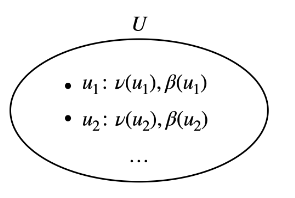
\includegraphics[width=0.5\textwidth]{../assets/discrete-money-distribution.png}
    \caption{Schematic representation of discrete money distribution}
    \label{fig:discrete-md}
\end{figure}

\subsubsection{Using Context}

But the discrete nature of the model does not provide the necessary element for us to add the desired properties to the
payment system. Here we propose a modification that involves the usage of \textit{context ($\gamma$)}:

\begin{figure}[h]
    \centering
    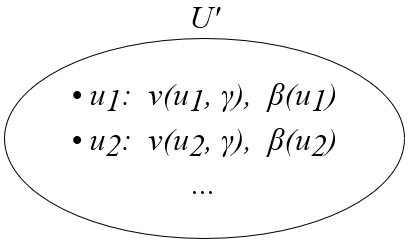
\includegraphics[width=0.5\textwidth]{../assets/money-distribution-with-ctx.png}
    \caption{Schematic representation of money distribution with context}
    \label{fig:md-with-ctx}
\end{figure}

Note that in this model, context can be updated independently while value functions of the same money distribution can
produce different monetary values.

\paragraph{Components of Context}

Here are some possible components of context, and how they work:

\begin{itemize}
\item If time (t) is included the context, then monetary value of each monetary unit can be continuous over time. Time
    is part of the physical reality, hence not changeable by the actors in the payment system.
\item Any subset of monetary units can also have their value functions depending on the same information in
    context. This could enable payment primitives that involve many parties. This set of information in context is
    referred to as \textit{ctx :: SharedContext}, they can be changed over time by the actors in the payment system.
\end{itemize}

For the purpose of this paper, the model of context is: $\gamma = (t :: Timestamp) \oplus (ctx :: SharedContext)$.

\subsubsection{Haskell Definition Of Money Distribution}

\input{MoneyDistribution.lhs.tex}


\subsection{Payment Primitives}
%%%%%%%%%%%%%%%%%%%%%%%%%%%%%%%

Payment primitives are functions that takes a money distribution, shared context, some payment instruction (args) and
timestamp as inputs and incremental updates\footnote{Specifically being monoidal, that is in short a set that has
associative binary operation and an identity element. See https://ncatlab.org/nlab/show/monoid. } of money
distribution and shared context as outputs:

\begin{minted}[escapeinside=||,mathescape=true]{haskell}
    somePaymentPrimitive :: ( Timestamp t
                            , MoneyDistribution md
                            , SharedContext ctx
                            , PaymentInstruction args
                            , Monoid md, Monoid ctx
                            )
                         => md |$\times$| ctx -> args -> t -> md |$\times$| ctx
\end{minted}

Loosely speaking, it is considered a primitive, if it can not be broken down into other existing primitives which result
in the same money distribution; additionally primitives should be the only constructs in a payment system that can
update money distribution.

Updates are \textit{monoidal}, so that they can be incremental and their parallel executions can be modeled.

The best known primitive is instant transfer of monetary value between one monetary unit to another. The introduction of
context enables more primitives to be defined, and this will be discussed in later chapters.


\subsection{Payment Execution Environment}
%%%%%%%%%%%%%%%%%%%%%%%%%%%%%%%%%%%%%%%%%%

The purpose of a payment execution environment is to perform the actual payment primitives, where their computation
interface, parallel evaluation strategies and payment system solvency are defined.

It is out of scope for this paper to survey in-depth the problem space of the operation semantics of payment execution
environments. Nonetheless, a simplified model and some potential extensions to it is discussed briefly.

\subsubsection{Composing Financial Contracts}

\input{FinancialContract.lhs.tex}

\subsubsection{Simplified Execution Environment Models}

\input{PaymentExecutionEnvironment.lhs.tex}


\subsection{Payment System Solvency}

While money distribution does not assign meaning to the range of monetary values, in real world applications, negative
values can have special meanings. In the following analysis, we call any money unit that has a negative monetary value
insolvent.

The detailed analysis of these solvency models are out of scope for this paper.

\paragraph{Buffer Based Solvency Treatment}

In a nondeterministic execution environment, we cannot determine when any financial contract will actually be
executed. That means, there is always a chance a monetary unit could reach negative monetary value.

To mitigate this uncertainty, a concept called buffer is introduced. A buffer has a monetary value which is set aside in a solvency conditional financial contract, such that if a solvency
condition arises, the buffer maybe drawn to cover the loss introduced by the nondeterministic timing of the execution.

\paragraph{Deterministic Solvency Treatment}

Since \textit{fcNext} returns what is the next financial contract executable at a specific time, this deterministic
property eliminates the need for the buffer.

But it introduces a different type of systemic risk, that is denial-of-service, since the system cannot advance the
system time until all next executable contracts are executed.


\subsection{Money Mediums}
%%%%%%%%%%%%%%%%%%%%%%%%%%%%%%%%

\begin{displayquote}
A useful observation about existing money schemes is that they all have some kind of monetary units that are physical or
digital representations of money. Examples are bills, coins, bank accounts, Bitcoin UTXOs,
etc. \footfullcite[][P3]{buldas2021unifying}
\end{displayquote}

We call them money mediums, and we further separate them into two big groups:

\begin{itemize}
\item \textit{Token and its Accounts} - \eg\ bank currency accounts. Each token is its own centralized execution
    environment, bearers access their monetary value through their accounts, and execute financial contracts through the
    token.
\item \textit{Note} - \eg\ federal reserve notes, bills, coins and Bitcoin UTXOs, etc. The execution environment is
    independent of the notes, but it needs notes to complete the execution of financial contracts.
\end{itemize}

One of the main differences is from the ``user interface'' perspective. A bearer expects to keep many notes at hand,
while maybe only needs a few accounts for each token. Also it is up to bearers to keep track of all their notes, while
token can keep track of most of the states for bearers; hence notes are more decentralized and tokens are more
centralized. Some also argue note-like model is better for complex concurrent and distributed computing environment
\footfullcite[][P2]{chakravarty2020extended}.

\subsubsection{Haskell Definition Of Money Mediums}

\input{MoneyMedium.lhs.tex}


%%%%%%%%%%%%%%%%%%%%%%%%%%%%%
\section{Relevant Approaches}
%%%%%%%%%%%%%%%%%%%%%%%%%%%%%

The focus of this paper is to formally define a set of payment primitives that modernize our payment systems. To prevent
reinventing wheels, it is relevant to discuss first some approaches in computer science that are believed to help
solving this challenge.

\subsection{Functional Reactive Programming}
%%%%%%%%%%%%%%%%%%%%%%%%%%%%%%%%%%%%%%%%%%%%

Recall that we want our modernized payment system to handle money distribution continuously over time, and its financial
contracts compositional. A very closely related software design paradigm best known to address those needs is
\textit{functional reactive programming (FRP)}. It was first introduced by Conal Elliott \& Paul Hudak in solving
multimedia animations \cite{elliott1997functional}. Later on, Hudak also worked on \cite{hudak2002arrows} and
\cite{wan2000functional} making FRP a more general framework for programming hybrid system with continuous behaviors in
a high-level, declarative manner.

After FRP got more adoption, it evolved to some variations that support discrete semantics, and some variations better
suited more for interactive systems. In this paper we will stick to and revisit the basic constructions of the original
formulation used in \cite{elliott1997functional} where we will draw inspirations from.

\paragraph{Temporal Modeling and Behaviors}

Values that vary over continuous time are called \textit{behaviors}. They are first-class values, and are built up
compositionally. In modern payment systems, we should want the monetary values of monetary units capable of varying over
continuous time. The semantic function of $\alpha$-behaviors produces the value of type $\alpha$ of a behavior at a given
time:

\begin{equation}
    at : Behavior_{\alpha} \rightarrow Time \rightarrow \alpha
\end{equation}

\paragraph{Event Modeling}

Like behaviors, \textit{events} are first-class values too. The semantic function of $\alpha$-event describes the time and
information associated with an \textit{occurrence} of the event:

\begin{equation}
    occ : Event_{\alpha} \rightarrow Time \times \alpha
\end{equation}

In modern payment systems, the payment primitives executed in payment execution environments are one type of
events. More types of events can be read from the original paper \footfullcite[][section 2.3 Semantics of
    Events]{elliott1997functional}.

\paragraph{Reactivity}

They key to modeling the payment execution environment using FRP is the \textit{reactivity}, which makes behaviors
reactive. Specifically, the behavior \textit{b untilB e} exhibits b's behavior until \textit{e} occurs, and then swiches
to a new behavior encoded in \textit{e}:

\begin{equation}
    \begin{split}
    &untilB : Behavior_{\alpha} \rightarrow Event_{Behavior_{\alpha}} \rightarrow Behavior_{\alpha} \\
    &at\ [\![b\ until\ B]\!]\ t = if\ t\ \leq\ t_{e}\ then\ at\ [\![b]\!]\ t\ else\ at\ [\![b']\!]\ t \\
    &\qquad where (t_e, b') = occ[\![e]\!]
    \end{split}
\end{equation}

Note that $[\![.]\!]$ is the denotational semantics notation to be introduced later.

In the context of modern payment systems, the occurrences of payment primitives (events) change the behaviors of
monetary units in how much monetary values it has over continuous. The building blocks of the financial contracts should
be about modeling these events and their reactivity declaratively.

\subsection{Denotational Semantics}
%%%%%%%%%%%%%%%%%%%%%%%%%%%%%%%%%%%

We also want a formal and precise specification of payment primitives. The title of the paper contains
\textit{denotational semantics}: ``it is a \textit{compositional} style for precisely specifying the meanings of
languages, invented by Christopher Strachey and Dana Scott in the 1960s (\cite{scott1971toward})'', and Conal Elliott
proposed that denotational semantics can also be applied to \textit{data types} in programming \footfullcite[][section
    2, denotational semantics and data types]{Elliott2009-type-class-morphisms-TR}. We will revisit this formulation
too.

... TODO

%%%%%%%%%%%%%%%%%%%%%%%%%%%%%%%%%%%%%%%%%%%%%%%%%%%%%%%%%%%%%%%%%%%%%%%%%%%%%%%%%%%%%%%%%%%%%%%%%%%%%%%%%%%%%%%%%%%%%%%%
\chapter{General Payment Primitives}
%%%%%%%%%%%%%%%%%%%%%%%%%%%%%%%%%%%%%%%%%%%%%%%%%%%%%%%%%%%%%%%%%%%%%%%%%%%%%%%%%%%%%%%%%%%%%%%%%%%%%%%%%%%%%%%%%%%%%%%%

%%%%%%%%%%%%%%%%%%%%%%%%%%%%%%%%
\section{Denotational Semantics}
%%%%%%%%%%%%%%%%%%%%%%%%%%%%%%%%

Here is the specification of denotational semantics that support both discrete and continous payments.

Here is the list of acronyms used:

\begin{itemize}
    \item \textbf{MD} is \textit{Money Distribution}.
    \item \textbf{MU} is \textit{Monetary Unit}.
    \item \textbf{RTB} is \textit{Real Time Balance}.
\end{itemize}

\subsection{Generalized Payment Model}

\begin{equation}\label{sem_transfer}
    \begin{split}
        [\![MD\ mu\ t\ rtb]\!] = mu \rightarrow t \rightarrow rtb
    \end{split}
\end{equation}

\subsection{Monoidial Payment Model}
%%%%%%%%%%%%%%%%%%%%%%%%%%%%%%%%%%%%

\begin{equation}\label{sem_mzero}
    [\![\emptyset]\!] = \lambda\ mu\ t\ \rightarrow 0
\end{equation}

\begin{equation}\label{sem_mappend}
    [\![mda \oplus\ mdb]\!] = \lambda\ mu\ t\ \rightarrow
    [\![mda]\!]\ mu\ t\ +\ [\![mdb]\!]\ mu\ t
\end{equation}

\subsection{Payment Primitives}
%%%%%%%%%%%%%%%%%%%%%%%%%%%%%%%

\begin{equation}\label{sem_transfer}
    \begin{split}
        [\![&transfer\ from\ to\ amount\ md]\!] = [\![md]\!]\ \oplus \\
        (\lambda\ case&\ mu\ t \\
        &|\ from = mu \rightarrow -amount \\
        &|\ to   = mu \rightarrow amount \\
        &|\ otherwise \rightarrow 0 \\
        )
    \end{split}
\end{equation}

\begin{equation}\label{sem_updateConstantFlow}
    \begin{split}
        [\![&updateConstantFlow\ from\ to\ flowRate\ t'\ md]\!] = [\![md]\!]\ \oplus \\
        (\lambda\ case&\ mu\ t \\
        &|\ from = mu \rightarrow -flowRate * (t - t') \\
        &|\ to   = mu \rightarrow flowRate  * (t - t') \\
        &|\ otherwise \rightarrow 0 \\
        )
    \end{split}
\end{equation}

\begin{equation}
    unit :: sub \rightarrow subs \rightarrow Int
\end{equation}

\begin{equation}
    proportion\ sub\ subs = {{ unit\ sub\ subs } \over { \displaystyle \sum_{x \in subs} unit\ x\ subs }}
\end{equation}

\begin{equation}\label{sem_distributeProportionally}
    \begin{split}
        [\![&distributeProportionally\ pub\ subs\ amount\ md]\!] = [\![md]\!]\ \oplus \\
        (\lambda\ case&\ mu\ t \\
        &|\ pub = mu \rightarrow -amount \\
        &|\ \exists sub \in subs\ { sub = mu } \rightarrow amount * (proportion\ mu\ subs) \\
        &|\ otherwise \rightarrow 0 \\
        )
    \end{split}
\end{equation}

\begin{equation}\label{sem_distributeProportionally}
    \begin{split}
        [\![&updateProportionalDistributionConstantFlow\ pub\ subs\ flowRate\ t'\ md]\!] = [\![md]\!]\ \oplus \\
        (\lambda\ case&\ mu\ t \\
        &|\ pub = mu \rightarrow -flowRate * (t - t') \\
        &|\ \exists sub \in subs\ { sub = mu } \rightarrow flowRate * (t - t') * (proportion\ mu\ subs) \\
        &|\ otherwise \rightarrow 0 \\
        )
    \end{split}
\end{equation}

%%%%%%%%%%%%%%%%%%%%%%%%%%%%%%%%
\section{Restatement in Haskell}
%%%%%%%%%%%%%%%%%%%%%%%%%%%%%%%%

%%%%%%%%%%%%%%%%%%%%%%%%%%%%%%%%%%%%%%%%%%%%%%%%%%%%%%%%%%%%%%%%%%%%%%%%%%%%%%%%%%%%%%%%%%%%%%%%%%%%%%%%%%%%%%%%%%%%%%%%
\chapter{Superfluid Money - A Reference Implementation}
%%%%%%%%%%%%%%%%%%%%%%%%%%%%%%%%%%%%%%%%%%%%%%%%%%%%%%%%%%%%%%%%%%%%%%%%%%%%%%%%%%%%%%%%%%%%%%%%%%%%%%%%%%%%%%%%%%%%%%%%

\section{Real Time Balance}

\section{Sub Systems}

\section{Agreement Sub System}

\section{Type of Agreements}

\subsection{Transferable Balance Agreement}

\subsection{Constant Flow Agreement}

\subsection{Distribution Agreement}

\subsection{Decaying Flow Agreement}

\section{Solvency Sub Systems}

\subsection{Buffer Based Solvency Systems}

\section{Type Of Monetary Units}

%%%%%%%%%%%%%%%%%%%%%%%%%%%%%%%%%%%%%%%%%%%%%%%%%%%%%%%%%%%%%%%%%%%%%%%%%%%%%%%%%%%%%%%%%%%%%%%%%%%%%%%%%%%%%%%%%%%%%%%%
\chapter{Future Investigations}
%%%%%%%%%%%%%%%%%%%%%%%%%%%%%%%%%%%%%%%%%%%%%%%%%%%%%%%%%%%%%%%%%%%%%%%%%%%%%%%%%%%%%%%%%%%%%%%%%%%%%%%%%%%%%%%%%%%%%%%%

\section{Restatement in Agda and Correctness Proof}

\section{Payment in General Accounting Domains}

%%%%%%%%%%%%%%%%%%%%%%%%%%%%%%%%%%%%%%%%%%%%%%%%%%%%%%%%%%%%%%%%%%%%%%%%%%%%%%%%%%%%%%%%%%%%%%%%%%%%%%%%%%%%%%%%%%%%%%%%
\newpage
\printbibliography{}
%%%%%%%%%%%%%%%%%%%%%%%%%%%%%%%%%%%%%%%%%%%%%%%%%%%%%%%%%%%%%%%%%%%%%%%%%%%%%%%%%%%%%%%%%%%%%%%%%%%%%%%%%%%%%%%%%%%%%%%%

\end{document}
